\documentclass[11pt,a4paper]{ctexart}
\usepackage[margin=1.8cm]{geometry}
\usepackage{amsmath,amssymb,bm}
\usepackage{booktabs,graphicx,xcolor,hyperref,array,float}
\hypersetup{colorlinks=true,linkcolor=blue,urlcolor=blue,citecolor=blue}
\setlength{\parindent}{2em}
\setlength{\parskip}{0.22em}
\newcommand{\norm}[1]{\left\lVert #1\right\rVert}
\newcommand{\R}{\mathbb{R}}
\title{TU Delft 同数据集 IMU--UWB 定位精度调研\\
Task06、当前两滤波器 InEKF 与公开 MHE 的口径审计}
\author{同数据集文献复核、数学对照与真实结果比较}
\date{2026年8月3日}

\begin{document}
\pagestyle{plain}
\maketitle

\begin{abstract}
Task06 使用 TU Delft 「UWB dataset v1」的全部 12 条 TWR 日志。
严格检索数据 DOI、日志文件名和论文数据引用后，可核实的同数据定量研究
主要是 Pfeiffer 等人的 2021 RA-L 原论文，以及同团队 2023 IMAV/
2025 IJMAV 改进 MHE。论文在 8 锚点处给出的平均三维位置 RMSE 图读数
约为 $0.20$ m（MHE）和 $0.23$--$0.27$ m（EKF）。但作者 2021 公开
复现实验同时把 OptiTrack 高度加噪后作为高度量测，并用 OptiTrack 真值
残差窗口设置 UWB/高度量测标准差，故该结果不是纯 raw-IMU/raw-TWR
盲测。本项目当前 proposed deep 在零初差下的全程位置 RMSE 中位/均值为
$0.332/0.350$ m，在 $[6,-6,3]^\top$ m 初差下为 $0.356/0.362$ m，
两种初值共 24 次均收敛。表面精度尚未达到论文 oracle-aided 的
$\sim0.20$ m，但相对 Task06 原增广法分别改善 $17.9\%$ 和 $12.6\%$，
且提供了论文没有报告的 9 m 初始位置误差捕获证据。
补充分轴批测表明，本项目 nominal 全程的 $x/y/z$ RMSE 均值为
$0.095/0.086/0.324$ m，垂直误差贡献约 $85.2\%$ 的三维平方误差；
作者注入的 OptiTrack 高度伪量测自身预期噪声 RMS 仅约 $0.019$ m。
因此当前表面差距首先是高度信息量和评估协议差异，而非已经证实的
MHE 与 InEKF 数学形式净差距。
\end{abstract}

\section{数据集与检索边界}

数据集 DOI 为
\href{https://doi.org/10.4121/14827680.v1}{10.4121/14827680.v1}，
由 Crazyflie 2.1 在 TU Delft Cyberzoo 采集，包含 8 个 DWM1000 锚点、
三轴 IMU、TWR/TDoA 和 OptiTrack 三维位置。六类轨迹为 square、triangle、
octagon、hourglass、star 和 random；每类有两条 TWR 日志，共 12 条。

本调研只纳入明确引用该数据条目，或逐项说明并实际回放这组 Cyberzoo
日志的研究。仅引用 2021 论文、仅使用相同硬件、使用 UTIL、NTU VIRAL
等其他数据集的论文不计入同数据结果。可核实论文形成同一作者研究链：
\begin{enumerate}
 \item 2021 RA-L：数据集原始配套论文\cite{pfeiffer2021}；
 \item 2023 IMAV：动态步长和开关变量改进 MHE\cite{pfeiffer2023}；
 \item 2025 IJMAV：2023 工作的扩展期刊版\cite{pfeiffer2025}。
\end{enumerate}
未找到独立第三方团队在全部 12 条 TWR 日志上公开可复核的同口径 RMSE。
数据引用元数据并不完整，因此这里只声称「截至当前检索可核实」，不声称
绝对穷尽未被索引的论文。

\section{论文方法与公开评估协议}

\subsection{六维 MHE 与本项目 15 维 InEKF 的状态差异}

Pfeiffer 等人的 MHE 优化六维位置/体轴速度状态
\begin{equation}
 \xi=[x^\top,\rho^\top]^\top\in\R^6,
\end{equation}
姿态由互补滤波器给出，IMU 导出的姿态、角速度和总推力作为系统输入。
其输出误差 MHE 在长度为 $N+1$ 的窗口中近似最小化
\begin{equation}
 J_t(\hat\xi_{t-N})=
 \mu\norm{\hat\xi_{t-N}-\bar\xi_{t-N}}^2+
 \sum_{k=t-N}^{t}\sum_i
 \theta_{i,k}\norm{y_{i,k}-H_{i,k}(\hat\xi_{t-N})}^2,
\end{equation}
并且每个时刻只执行一次梯度、线搜索或 Newton 更新。

本项目 tracker 的误差状态为
\begin{equation}
 \delta x_{\rm tr}=
 [\delta\theta^\top,\delta v^\top,\delta p^\top,
  \delta b_g^\top,\delta b_a^\top]^\top\in\R^{15}.
\end{equation}
原始 TWR 创新为
\begin{align}
 \nu_i&=(\rho_i^m-b_\rho)-\norm{a_i-\hat p^-},\\
 K_i&=P^-H_i^\top(H_iP^-H_i^\top+\sigma_\rho^2)^{-1},
\end{align}
UWB 可通过传播形成的交叉协方差修正速度、姿态和 IMU 偏置。capture
支路另维护
\begin{equation}
 \chi=[q,s,h,p^\top,v^\top,1]^\top,
 \quad q=\tfrac12p^\top p,\ s=p^\top v,\ h=v^\top v,
\end{equation}
利用估计状态无关的平方距离观测行扩大大初差捕获域。当前 deep 输出由
健康监督器在 capture 与 tracker 之间因果交接，二者承担的任务不等同于
论文六维 MHE。

\subsection{公开 2021 复现代码中的真值辅助}

论文锚点批测脚本明确设置
\begin{equation}
 \texttt{altitude\_enable=True}.
\end{equation}
数据回放代码以 OptiTrack 高度构造
\begin{equation}
 y_{z,k}=z_k^{\rm OT}(1+\epsilon_k),
 \qquad \epsilon_k\sim\mathcal N(0,0.02^2),
 \label{eq:oracle-alt}
\end{equation}
并以真值位置形成每个锚点的距离误差
\begin{equation}
 e_{i,k}^{\rho}=\rho_{i,k}^m-\norm{a_i-p_k^{\rm OT}},
 \qquad
 \sigma_{i,k}=\operatorname{Std}
 \{e_{i,j}^{\rho}\}_{j=k-9}^{k},
 \label{eq:oracle-sigma}
\end{equation}
再把 $\sigma_{i,k}$ 交给估计器。式\eqref{eq:oracle-alt} 是连续真值高度
伪量测，式\eqref{eq:oracle-sigma} 是真值依赖的量测权重。对应文件是论文
时期提交，而非后来偏离论文的改动\cite{codeanchors,codedrone}。

因此论文实验可准确表述为「真实 IMU、真实 TWR，加 OptiTrack 派生高度和
真值辅助量测噪声」。把其 $\sim0.20$ m 简化称为纯 IMU+UWB 精度会遗漏
决定性的评价条件。

\section{同数据集论文精度}

\begin{table}[H]
\centering
\small
\caption{公开论文在全部 8 锚点 TWR 处的图读数。论文未给数值表，故只报
$\sim0.01$ m 精度。}
\begin{tabular}{p{2.2cm}p{4.2cm}p{3.2cm}p{2.2cm}}
\toprule
研究 & 数据和统计 & 8 锚点位置 RMSE & 成功率\\
\midrule
RA-L 2021 & 12 条 TWR，每条每个锚点数 10 次；成功阈值 1 m；只对成功运行求均值
& EKF $\sim0.23$ m；MHE $\sim0.20$ m & 100\%\\
IMAV 2023 & 12 条 TWR、10 个随机种子；成功阈值 0.5 m；失败从精度统计移除
& EKF $\sim0.27$ m；MHE 变体 $\sim0.20$--$0.21$ m & 100\%\\
IJMAV 2025 & 2023 工作的扩展期刊版，同数据、同实验系列
& 与 2023 同量级 & 100\%\\
\bottomrule
\end{tabular}
\end{table}

2023/2025 比较简单梯度、线搜索和 Newton 法，以及 RANSAC/SVOR 两种
离群处理。MHE 变体之间的精度曲线几乎重合；改进主要体现为锚点数量变化时
的鲁棒性和计算负荷，而不是把 8 锚点 RMSE 显著降到 $0.20$ m 以下。

\section{本项目当前结果及相对 Task06 的变化}

当前正式结果对同一行 IMU/TWR 共同使用
\begin{equation}
 t_k^{\rm acquisition}=t_k^{\rm log}-0.20\ \mathrm{s},
\end{equation}
并在采集时刻插值 OptiTrack 用于评价。该时延由本数据集标定，因此同样是
描述性而非独立盲测参数，但 OptiTrack 位置没有作为滤波量测注入。

\begin{table}[H]
\centering
\small
\caption{12 条 TWR 日志的全程三维位置 RMSE。large 初差
$[6,-6,3]^\top$ m 的范数准确为 9 m。}
\begin{tabular}{llrrrr}
\toprule
阶段 & 初值 & 中位数 (m) & 均值 (m) & 末5 s中位 (m) & 收敛\\
\midrule
Task06 松耦合增广 & nominal & 0.404446 & 0.401514 & 0.334650 & 12/12\\
当前 proposed deep & nominal & 0.331862 & 0.349604 & 0.211725 & 12/12\\
Task06 松耦合增广 & large & 0.407519 & 0.408992 & 0.334650 & 12/12\\
当前 proposed deep & large & 0.356247 & 0.362371 & 0.211746 & 12/12\\
当前 proposed deep & 合并24次 & 0.338625 & 0.355987 & 0.211746 & 24/24\\
\bottomrule
\end{tabular}
\end{table}

相对 Task06 原增广法，当前 deep 的全程中位数改善为
\begin{align}
 \Delta_{\rm nominal}
 &=\frac{0.331862-0.404446}{0.404446}=-17.9\%,\\
 \Delta_{\rm large}
 &=\frac{0.356247-0.407519}{0.407519}=-12.6\%.
\end{align}
当前 ordinary InEKF 在 nominal 下为 $0.322$ m 中位数，略优于 deep；
但 large 下只有 7/12 收敛，均值因真实发散达到 $84.23$ m。deep 的收益
是同时保留大初差捕获和稳定跟踪，而不是每个名义稳态指标都最小。

\begin{figure}[H]
\centering
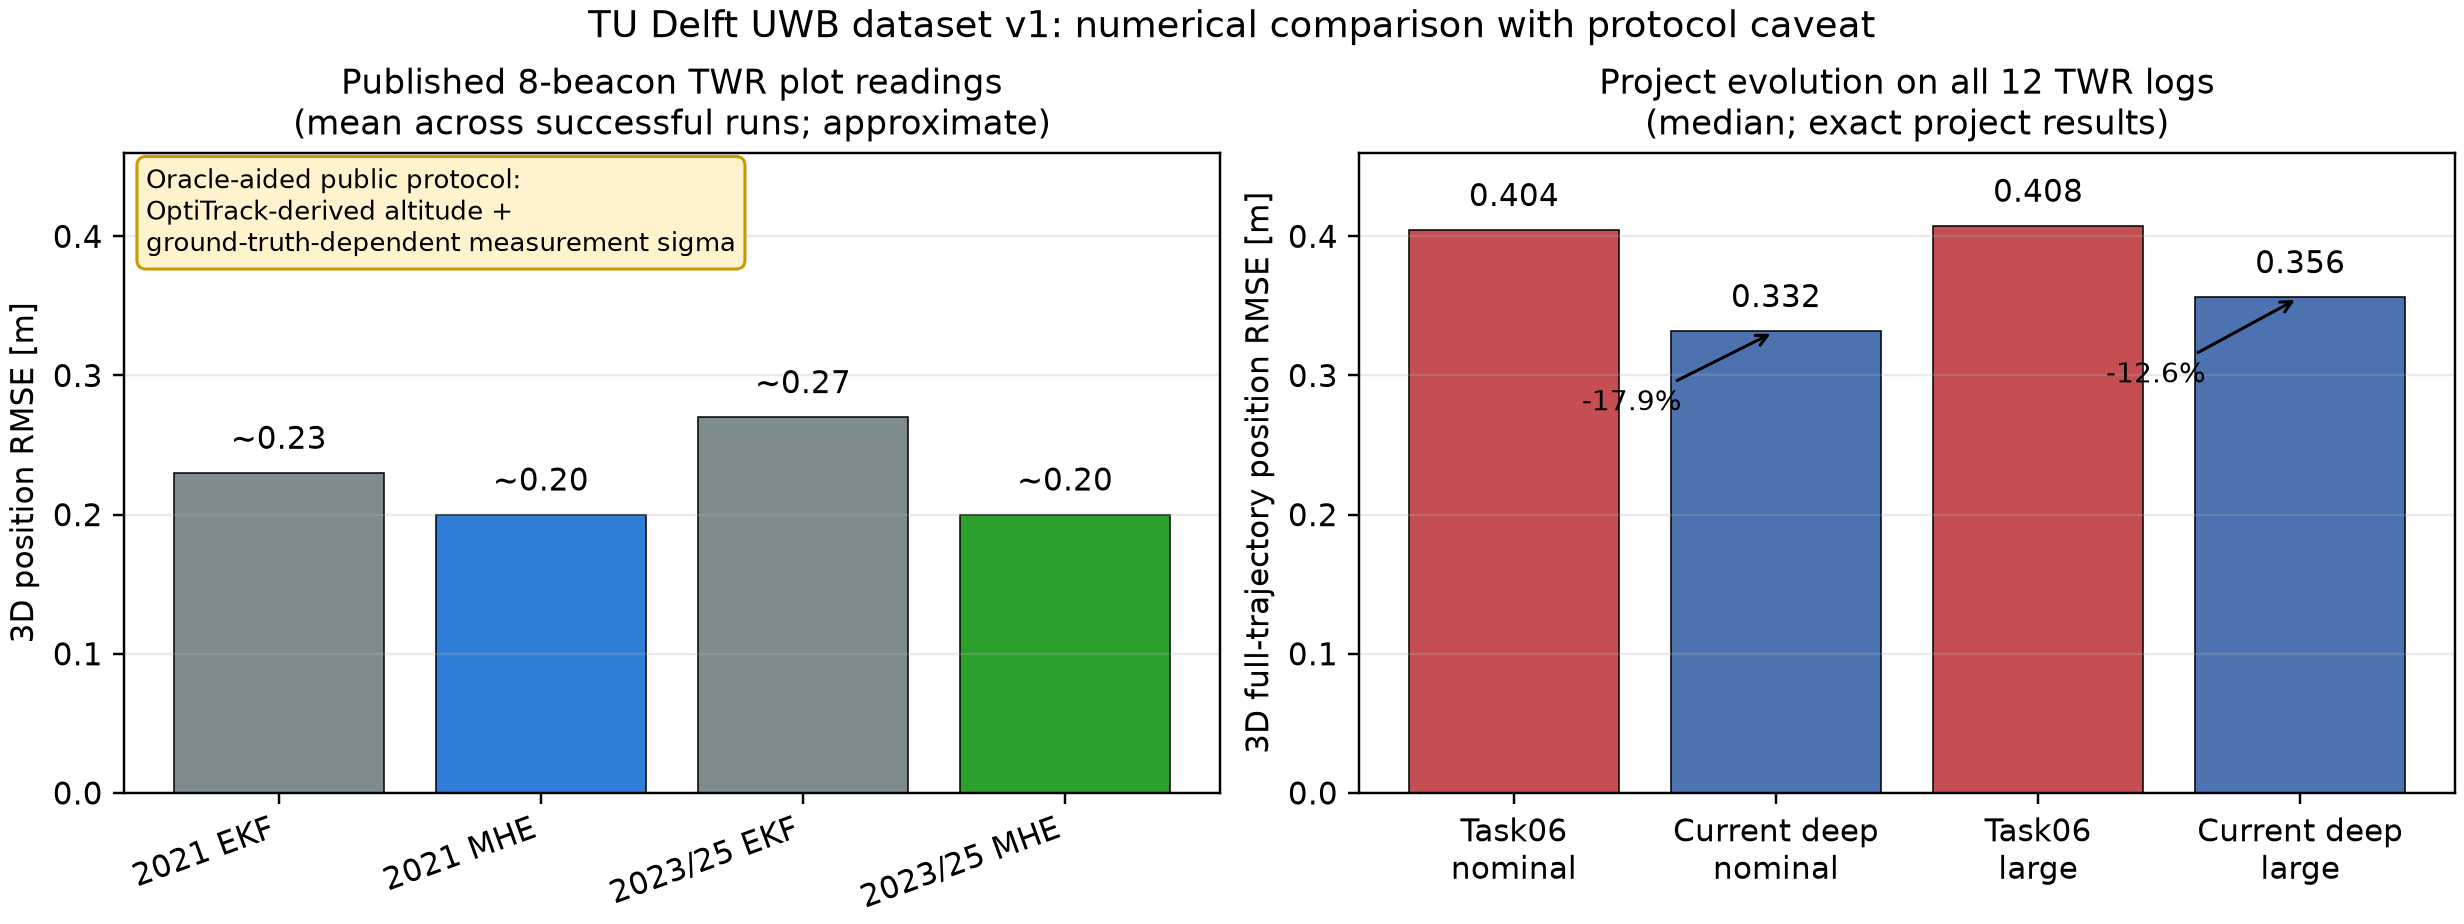
\includegraphics[width=0.98\textwidth]{task06_same_dataset_accuracy_comparison.png}
\caption{左：论文 8 锚点图读数，含真值辅助协议；右：本项目两阶段精确
中位数。两幅子图特意分开，避免把均值/中位数和不同输入协议混成公平排名。}
\end{figure}

\section{精度差距的分轴与因果分解}

\subsection{本项目误差主要在垂直方向}

在正式 $0.20$ s 共同 IMU/TWR 时延下，重新运行 12 条 nominal 日志，
对 deep 位置误差
\begin{equation}
 e_k=\hat p_k-p_k^{\rm OT}
\end{equation}
分别按坐标轴计算 RMSE，结果如下。该重放没有修改算法参数。

\begin{table}[H]
\centering
\small
\caption{当前 deep 的分轴误差。水平 RMSE 等价于仅在评分阶段把 $z$
设为精确真值后的反事实三维 RMSE。}
\begin{tabular}{lrrrrr}
\toprule
窗口 & 三维/m & $x$/m & $y$/m & $z$/m & $z$平方占比\\
\midrule
全程 & 0.3496 & 0.0950 & 0.0864 & 0.3239 & 85.2\%\\
去掉前1 s & 0.3506 & 0.0950 & 0.0867 & 0.3249 & 85.2\%\\
20 s以后 & 0.3461 & 0.0962 & 0.0897 & 0.3187 & 84.1\%\\
末5 s & 0.2180 & 0.1000 & 0.0546 & 0.1815 & 66.6\%\\
\bottomrule
\end{tabular}
\end{table}

全程水平 RMSE 均值只有 $0.12895$ m，而三维为 $0.34960$ m。这里
把 $z$ 换成真值仅用于误差归因，不代表一个可部署滤波器，也不能当作
本项目新成绩。但它证明垂直误差的量级足以覆盖表面 $0.15$ m 差距。

作者注入高度的条件标准差为 $0.02|z_k^{\rm OT}|$。本数据 12 条日志
的高度 RMS 为 $0.94201$ m，因此该伪传感器的预期噪声 RMS 为
\begin{equation}
 \sigma_{z,\rm rms}=0.02\sqrt{\frac1N\sum_k(z_k^{\rm OT})^2}
 =0.01884\ \mathrm{m}.
\end{equation}
它与本项目全程 $z$ RMSE 的 $0.32392$ m 相差一个数量级以上。去掉前1 s
或只看20 s以后均没有明显降低三维误差，说明 nominal 差距不是计分起点或
20 s capture 驻留造成的。

\begin{figure}[H]
\centering
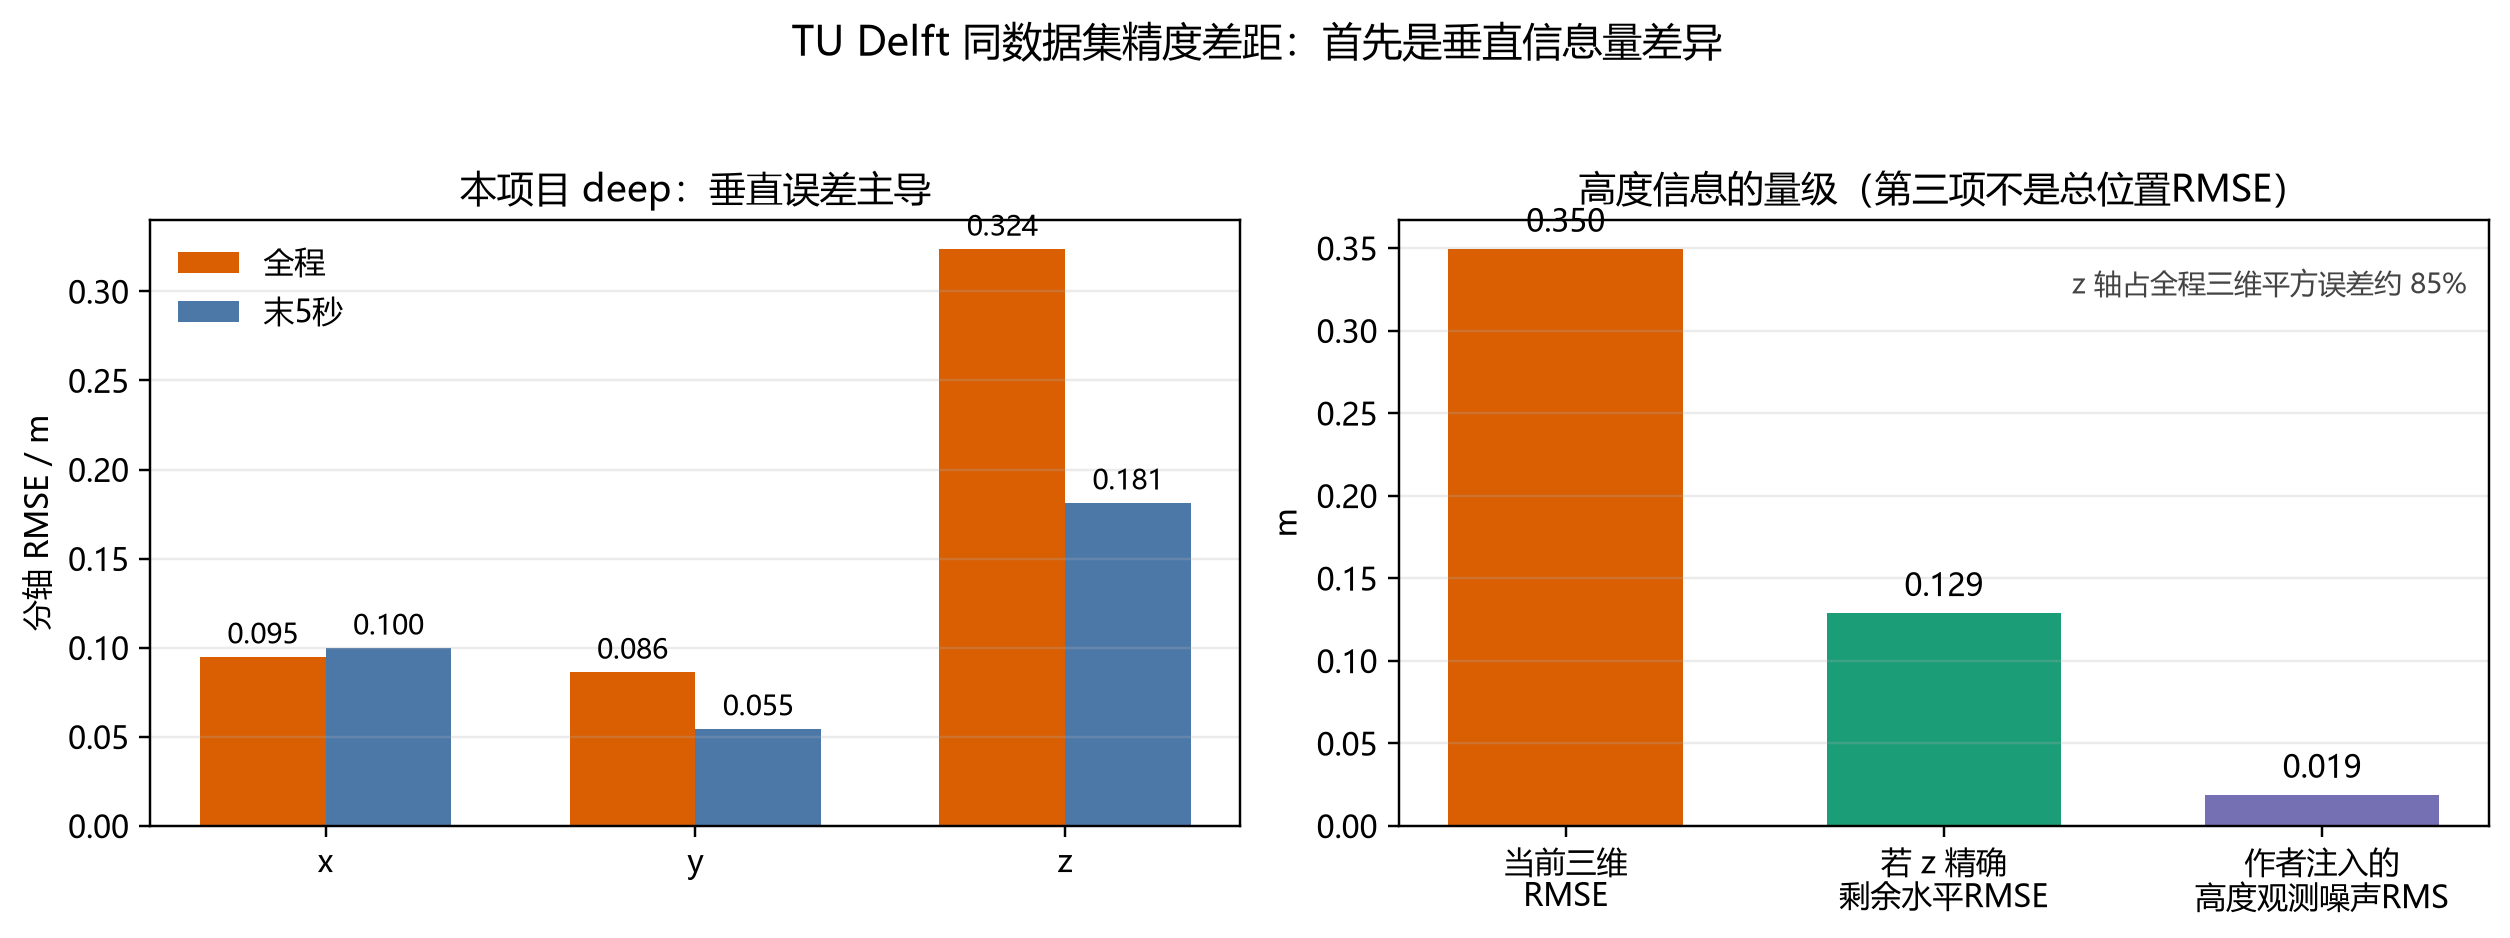
\includegraphics[width=0.98\textwidth]{task06_accuracy_gap_decomposition.png}
\caption{左：本项目分轴误差；右：三维、反事实精确高度后的水平误差及作者
注入高度观测的噪声量级。右图第三柱不是总位置 RMSE。}
\end{figure}

\subsection{为什么本项目的垂直方向更难估计}

以八锚点斜距观测矩阵
\begin{equation}
 H_i=\frac{(p-a_i)^\top}{\norm{p-a_i}}
\end{equation}
计算，当前轨迹上的中位单位测距噪声放大系数为
\begin{equation}
 \sqrt{\operatorname{diag}((H^TH)^{-1})}
 \simeq[0.511,0.510,2.059].
\end{equation}
垂直方向约为水平的4倍。论文正文也明确说明 UWB 单独估计高度通常困难，
因此引入专用高度观测；公开回放却以 OptiTrack 高度实现该观测。

当前时延对齐后共审计 148491 个 TWR 事件。全局 $-0.18$ m 校正后的残差
均值、标准差、RMSE 为 $0.00290/0.17727/0.17730$ m，但逐锚原始偏差均值
从 $-0.0654$ m 到 $-0.2590$ m，标准差从 $0.0835$ m 到 $0.2917$ m。
当前所有锚点仍共用一个偏差和标准差，不能描述这些差异。

当前 NIS 门限为25，24次运行每条日志拒绝数中位仅5.5，而接受量测约
$10^4$--$1.5\times10^4$ 次。故多数20--40 cm的多径/NLOS误差未超过
5-sigma硬门限，仍作为普通高斯观测进入滤波。论文 MHE 的滑窗、RANSAC及
后续开关变量能处理部分剩余误差，这是可信的算法优势；但论文同协议下
MHE 相对 EKF 只改善约3--7 cm，尚不能把全部表面差距归给滤波器类别。

\subsection{本项目也有数据集特定真值使用}

本项目 nominal 初始位置取第一帧 OptiTrack，固定距离偏差和 $0.20$ s
时延也在本数据上标定，监督阈值没有完全独立留出集。这些属于一次性初始化
和离线标定，不等同于在每个更新时刻读取答案，但说明本结果同样是描述性验证，
不能包装成跨数据集盲测。真正公平的算法消融必须同时关闭作者的连续真值高度
和真值权重，并统一双方的离线校准、初值及评分。

\section{可以和不可以下的结论}

若只按表面数字，以论文 MHE $0.20$ m 对比本项目 nominal deep 均值：
\begin{equation}
 \frac{0.349604-0.20}{0.20}=74.8\%.
\end{equation}
本项目尚未达到文献最低图示数字。但这个 $74.8\%$ 不能解释为算法净差距，
因为论文连续使用 OptiTrack 派生高度和真值依赖噪声；本项目还估计完整偏置
状态，并保留所有 9 m 大初差捕获瞬态。当前 deep 的末 5 s 中位数
$0.212$ m 虽接近论文全程 $\sim0.20$ m，窗口不同，也不能宣称已经达到论文精度。

可信结论为：
\begin{enumerate}
 \item 文献在其 oracle-aided 公开协议下达到约 $0.20$ m；
 \item 本项目 raw-IMU/raw-TWR 的全程稳定精度仍为 $0.33$--$0.36$ m；
 \item 当前方法相对 Task06 有 12.6\%--17.9\% 的实测改善，并保持 24/24
       收敛；
 \item 文献没有给出 9 m 初差下的同口径结果，不能比较捕获鲁棒性；
 \item 真正的算法排名必须关闭作者代码的真值高度与真值噪声权重，并统一
       时延、初值、计分起点和均值/中位数统计。
\end{enumerate}

\section{复核状态}

本轮没有修改估计算法或重新调参；另以正式参数重放 12 条 nominal 日志完成
分轴和时间窗口审计，墙钟约84 s。当前正式 CSV/JSON 已复核；五方法
24 次散点图和代表性 9 m 初差轨迹已按原分辨率
检查。deep 轨迹连续有限，ordinary InEKF 的离群发散在对数坐标中完整保留，
没有用中位数、裁图或删失败运行美化结果。

\begingroup
\raggedright
\begin{thebibliography}{9}
\bibitem{dataset}
Pfeiffer, S., de Wagter, C., and de Croon, G.C.H.E.,
「Data underlying the publication: A Computationally Efficient Moving Horizon
Estimator for UWB Localization on Small Quadrotors,」 2021,
\href{https://doi.org/10.4121/14827680.v1}{doi:10.4121/14827680.v1}.

\bibitem{pfeiffer2021}
Pfeiffer, S., de Wagter, C., and de Croon, G.C.H.E.,
「A Computationally Efficient Moving Horizon Estimator for Ultra-Wideband
Localization on Small Quadrotors,」 IEEE Robotics and Automation Letters,
6(4):6725--6732, 2021,
\href{https://doi.org/10.1109/LRA.2021.3095519}{doi:10.1109/LRA.2021.3095519}.

\bibitem{pfeiffer2023}
Pfeiffer, S., de Wagter, C., and de Croon, G.C.H.E.,
「Improved Moving Horizon Estimation for Ultra-Wideband Localization on Small
Drones,」 IMAV 2023,
\url{https://www.imavs.org/papers/2023/10.pdf}.

\bibitem{pfeiffer2025}
Pfeiffer, S., de Wagter, C., and de Croon, G.C.H.E.,
「Improved moving horizon estimation for ultra-wideband localization on small
drones,」 International Journal of Micro Air Vehicles, 2025,
\href{https://doi.org/10.1177/17568293251340100}{doi:10.1177/17568293251340100}.

\bibitem{codeanchors}
Pfeiffer, S., publication anchor-count benchmark script, commit
\texttt{955360a8736c},
\url{https://github.com/SUPfeiffer/uwb-simulator/blob/955360a8736c/publication/headless_Nanchors.py}.

\bibitem{codedrone}
Pfeiffer, S., dataset replay and oracle measurement code, 「RAL2021 Full Code,」
commit \texttt{b43a7f6d9033},
\url{https://github.com/SUPfeiffer/uwb-simulator/blob/b43a7f6d9033/UWBsim/airframe/drone.py}.
\end{thebibliography}
\endgroup

\end{document}
